\subsubsection{UC\theuccount-PGL - Producer GitLab invia messaggio al Gestore Personale}
	\begin{figure}[H]
		\centering
		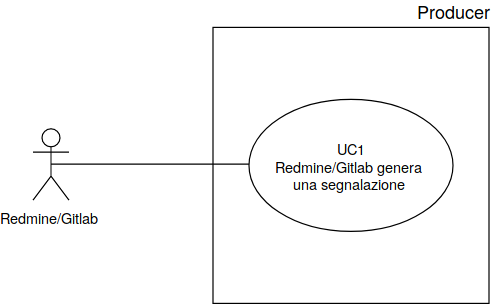
\includegraphics[width=0.7\textwidth]{img/UC1.png}\\
		\caption{UC\theuccount-PGL - Producer GitLab invia messaggio al Gestore Personale}
	\end{figure}
	\begin{itemize}
		\item \textbf{Codice}: UC\theuccount-PGL.
		\item \textbf{Titolo}: Producer GitLab invia messaggio al Gestore Personale.
		\item \textbf{Attori primari}: Producer GitLab.
		\item \textbf{Descrizione}: il sistema qui è Gestore Personale ed è interno al sistema Butterfly. Il Producer GitLab,
		dopo aver ricevuto una segnalazione da GitLab, elabora un messaggio da inviare al Gestore Personale.
		\item \textbf{Precondizione}: il Producer GitLab ha ricevuto una segnalazione da GitLab.
		\item \textbf{Postcondizione}: l Producer GitLab ha inviato al Gestore Personale il messaggio elaborato.
		\item \textbf{Scenario principale}: 
		\begin{enumerate}
			\item Producer GitLab procede all'invio del messaggio al Gestore Personale.
		\end{enumerate}
		
	\end{itemize}
	
	\paragraph{UC\theuccount.1-PGL - Producer GitLab invia uno o più messaggi di commit al Gestore Personale}
	\begin{figure}[H]
		\centering
		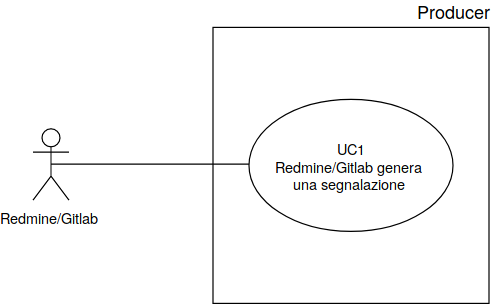
\includegraphics[width=0.7\textwidth]{img/UC1.png}\\
		\caption{UC\theuccount.1-PGL - Producer GitLab invia uno o più messaggi di commit al Gestore Personale}
	\end{figure}
	\begin{itemize}
		\item \textbf{Codice}: UC\theuccount.1-PGL.
		\item \textbf{Titolo}: Producer GitLab invia uno o più messaggi di commit al Gestore Personale.
		\item \textbf{Attori primari}: Producer GitLab.
		\item \textbf{Descrizione}: il sistema qui è Gestore Personale ed è interno al sistema Butterfly. Il Producer GitLab, dopo
		aver ricevuto una segnalazione di push da GitLab, elabora un messaggio per commit che verrà catalogato sotto il Topic "commits".
		Il messaggio elaborato conterrà i campi:
		\begin{itemize}
			\item Project
			\item Topic
			\item Message
		\end{itemize}
		\item \textbf{Precondizione}: il Producer GitLab ha ricevuto una segnalazione da GitLab.
		\item \textbf{Postcondizione}: il Producer GitLab ha inviato uno o più messaggi elaborati di commit.
		\item \textbf{Scenario principale}: 
		\begin{enumerate}
			\item Producer GitLab procede all'invio di uno o più messaggi
		 di commit al Gestore Personale.
		\end{enumerate}
		
	\end{itemize}

	\paragraph{UC\theuccount.2-PGL -  Producer GitLab invia messaggio di issue al Gestore Personale}
	\begin{figure}[H]
		\centering
		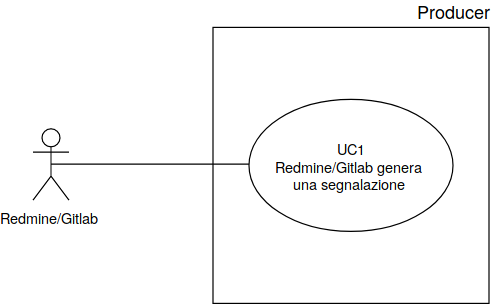
\includegraphics[width=0.7\textwidth]{img/UC1.png}\\
		\caption{UC\theuccount.2-PGL -  Producer GitLab invia messaggio di issue al Gestore Personale}
	\end{figure}
	\begin{itemize}
		\item \textbf{Codice}: UC\theuccount.2-PGL.
		\item \textbf{Titolo}:  Producer GitLab invia messaggio di issue al Gestore Personale.
		\item \textbf{Attori primari}: Producer GitLab.
		\item \textbf{Descrizione}: il sistema qui è Gestore Personale ed è interno al sistema Butterfly. Il Producer GitLab, dopo
		aver ricevuto una segnalazione di issue da GitLab, controlla se la issue è appena stata creata o si tratta di una modifica di
		una issue preesistente. Il messaggio elaborato, una volta elaborato, conterrà i campi:
		\begin{itemize}
			\item Project
			\item Topic
			\item Subject e opzionalmente:
			\begin{itemize}
				\item Description
				\item Due Date
				\item Milestone
				\item Assignee
			\end{itemize}
		\end{itemize}
		\item \textbf{Precondizione}: il Producer GitLab ha ricevuto una segnalazione da GitLab.
		\item \textbf{Postcondizione}: il Producer GitLab ha inviato al Gestore Personale il messaggio \newline elaborato.
		\item \textbf{Scenario principale}: 
		\begin{enumerate}
			\item Producer GitLab procede all'invio di un messaggio di
			issue al Gestore Personale.
		\end{enumerate}
		
	\end{itemize}
	
		\subparagraph{UC\theuccount.2.1-PGL - Producer GitLab invia messaggio di una nuova issue al Gestore Personale}
		\begin{figure}[H]
			\centering
			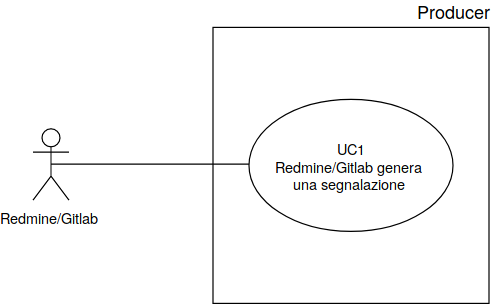
\includegraphics[width=0.7\textwidth]{img/UC1.png}\\
			\caption{UC\theuccount.2.1-PGL - Producer GitLab invia messaggio di una nuova issue al Gestore Personale}
		\end{figure}
		\begin{itemize}
			\item \textbf{Codice}: UC\theuccount.2.1-PGL.
			\item \textbf{Titolo}: Producer GitLab invia messaggio di una nuova issue al Gestore Personale.
			\item \textbf{Attori primari}: Producer GitLab.
			\item \textbf{Descrizione}: il sistema qui è Gestore Personale ed è interno al sistema Butterfly. Il Producer GitLab, dopo
			aver ricevuto una segnalazione di una nuova issue da GitLab, elabora il messaggio che conterrà i campi:
			\begin{itemize}
				\item Project
				\item Topic
				\item Subject e opzionalmente:
				\begin{itemize}
					\item Description
					\item Due Date
					\item Milestone
					\item Assignee
				\end{itemize}
			\end{itemize}
			\item \textbf{Precondizione}: il Producer GitLab ha ricevuto una segnalazione da GitLab.
			\item \textbf{Postcondizione}: il Producer GitLab ha inviato al Gestore Personale il messaggio elaborato di nuova issue.
			\item \textbf{Scenario principale}: 
			\begin{enumerate}
				\item Producer GitLab procede all'invio di un messaggio di
				nuova issue al Gestore Personale.
			\end{enumerate}
			
		\end{itemize}
	
		\subparagraph{UC\theuccount.2.2-PGL - Producer GitLab invia messaggio di modifica di una issue al Gestore Personale}
		\begin{figure}[H]
			\centering
			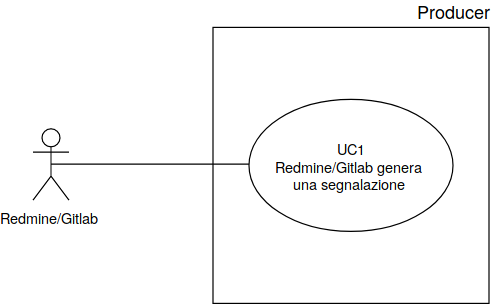
\includegraphics[width=0.7\textwidth]{img/UC1.png}\\
			\caption{UC\theuccount.2.2-PGL - Producer GitLab invia messaggio di modifica di una issue al Gestore Personale}
		\end{figure}
		\begin{itemize}
			\item \textbf{Codice}: UC\theuccount.2.2-PGL.
			\item \textbf{Titolo}: Producer GitLab invia messaggio di modifica di una issue al Gestore Personale.
			\item \textbf{Attori primari}: Producer GitLab.
			\item \textbf{Descrizione}: il sistema qui è Gestore Personale ed è interno al sistema Butterfly. l Producer GitLab, dopo
			aver ricevuto una segnalazione di modifica di una issue da GitLab, controlla se sono stati modificati i campi Label o Title.
			In caso positivo, viene inviato un messaggio elaborato al Gestore Personale, il quale conterrà:
			\begin{itemize}
				\item Project
				\item Topic
				\item Subject e opzionalmente:
				\begin{itemize}
					\item Description
					\item Due Date
					\item Milestone
					\item Assignee
				\end{itemize}
			\end{itemize}
			\item \textbf{Precondizione}: il Producer GitLab ha ricevuto una segnalazione da GitLab.
			\item \textbf{Postcondizione}: il Producer GitLab ha inviato al Gestore Personale il messaggio elaborato di modifica issue.
			\item \textbf{Scenario principale}: 
			\begin{enumerate}
				\item Producer GitLab procede all'invio di un messaggio di modifica issue al Gestore Personale.
			\end{enumerate}
			\item \textbf{Estensioni}: 
			\begin{enumerate}
				\item Ci sono dei messaggi non validi e vengono scartati [UCPGL\theuccount.2.3].
			\end{enumerate}
		\end{itemize}
	
		\subparagraph{UC\theuccount.2.3-PGL - Producer GitLab scarta i messaggi non validi}
		\begin{figure}[H]
			\centering
			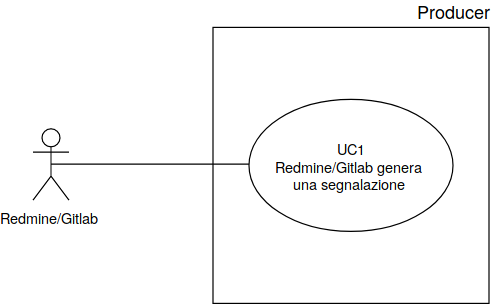
\includegraphics[width=0.7\textwidth]{img/UC1.png}\\
			\caption{UC\theuccount.2.3-PGL - Producer GitLab scarta i messaggi non validi}
		\end{figure}
		\begin{itemize}
			\item \textbf{Codice}: UC\theuccount.2.3-PGL.
			\item \textbf{Titolo}: Producer GitLab scarta i messaggi non validi.
			\item \textbf{Attori primari}: Producer GitLab.
			\item \textbf{Descrizione}: il Producer GitLab, dopo aver ricevuto una segnalazione di una modifica issue da GitLab, controlla
			se sono state modificati i campi Label o Title. In caso negativo, il messaggio viene scartato.
			\item \textbf{Precondizione}: il Producer GitLab ha ricevuto una segnalazione da GitLab.
			\item \textbf{Postcondizione}: il Producer GitLab ha scartato il messaggio.
			\item \textbf{Scenario principale}: 
			\begin{enumerate}
				\item Producer GitLab scarta i messaggi non validi.
			\end{enumerate}
		\end{itemize}